\documentclass[10pt,conference]{IEEEtran}

\ifCLASSOPTIONcompsoc
  \usepackage[nocompress]{cite}
\else
  \usepackage{cite}
\fi

% --- Graphic & Mathematics ---
\usepackage{graphicx}
\usepackage{amsmath,amsfonts}

% --- Algorithm & Tables ---
\usepackage{algorithmic}
\usepackage{algorithm}
\usepackage{array}
\usepackage{tabularx}
\usepackage{multirow}
\usepackage{booktabs}
\renewcommand{\arraystretch}{1.3}

% --- Color & Links ---
\usepackage[dvipsnames]{xcolor} 
\usepackage[
    colorlinks=true, 
    linkcolor=blue, 
    citecolor=blue,
    urlcolor=blue
]{hyperref}

% --- Code Highlight ---
\usepackage{minted}
\setminted{
    breaklines=true, 
    fontsize=\footnotesize, 
    linenos,
    frame=single,
    xleftmargin=1em,
    numbersep=5pt
}

% --- Section Style ---
\usepackage{titlesec}
\titleformat{\section}
{\normalfont\large\bfseries}
{\thesection}
{1em}
{}

\titleformat{\subsection}
{\normalfont\normalsize\bfseries}
{\thesubsection}
{1em}
{}

% --- Numbering Style ---
\renewcommand{\thesection}{\arabic{section}}
\renewcommand{\thesubsection}{\thesection.\arabic{subsection}}
\renewcommand{\thesubsubsection}{\thesubsection.\arabic{subsubsection}}

% --- Other Tools ---
\usepackage{url}
\ifCLASSOPTIONcompsoc
  \usepackage[caption=false,font=footnotesize,labelfont=sf,textfont=sf]{subfig}
\else
  \usepackage[caption=false,font=footnotesize]{subfig}
\fi

% --- Bibliography ---
\bibliographystyle{unsrt}

% --- User Info ---
\newcommand{\studentonename}{Shijia Luo}
\newcommand{\studenttwoname}{Yuwei Zhao}
\newcommand{\studentonenumber}{H00460252}
\newcommand{\studenttwonumber}{H00460398}
\newcommand{\labgroup}{CW2 Group19}
\newcommand{\labdate}{2026-05-10}
\newcommand{\course}{F28HS - Hardware-Software Interface}
\newcommand{\labtitle}{CW2 Report}

% --- Title ---
\title{
    \vspace{-1cm}
    \textbf{\labtitle}\\[0.3em]
    \Large \course
}
\author{
    \studentonename~(\studentonenumber)
    \quad
    \studenttwoname~(\studenttwonumber) \\[0.5em]
    \labgroup \quad \labdate
}
\date{}

\pagestyle{plain}

\begin{document}
    \maketitle
    \thispagestyle{plain}
    
    \section{Introduction}
\label{sec:introduction}

This purpose of this report is to clarify the development and analysis process of F28HS course programming project, the core of which is to develop an underlying system application program based on C and ARM assembly language, and run on the Raspberry Pi platform connected with external devices. The application aims at a deep understanding of the interactions between embedded hardware and external devices, and enables precise control of these interactions through the underlying code, covering resource management and time-sensitive operations.

In terms of the application implementation, the PinCrack password breaking system was successfully developed in this project, that is, we built a device that can accurately calculate and guess the secret PIN based on the proximity information between the guessed PIN and the correct PIN. The main interaction process of the system is the user inputs a sequence of numbers through a button as the input device, the Raspberry Pi will calculate the Hamming distance between the input sequence and the preset secret sequence, and return the alignment information through the LED flashing and the LCD display. The information provided by the Hamming distance is used as the pruning condition of the algorithm, and all possible values are efficiently searched to find the true secret sequence.

The following chapters will analyze and summarize the hardware connection, team division, code architecture, underlying hardware access interface and system performance.

    \section{Hardware Specification \& Wiring}
\label{sec:hardware_design}

\begin{figure}[H]
    \centering
    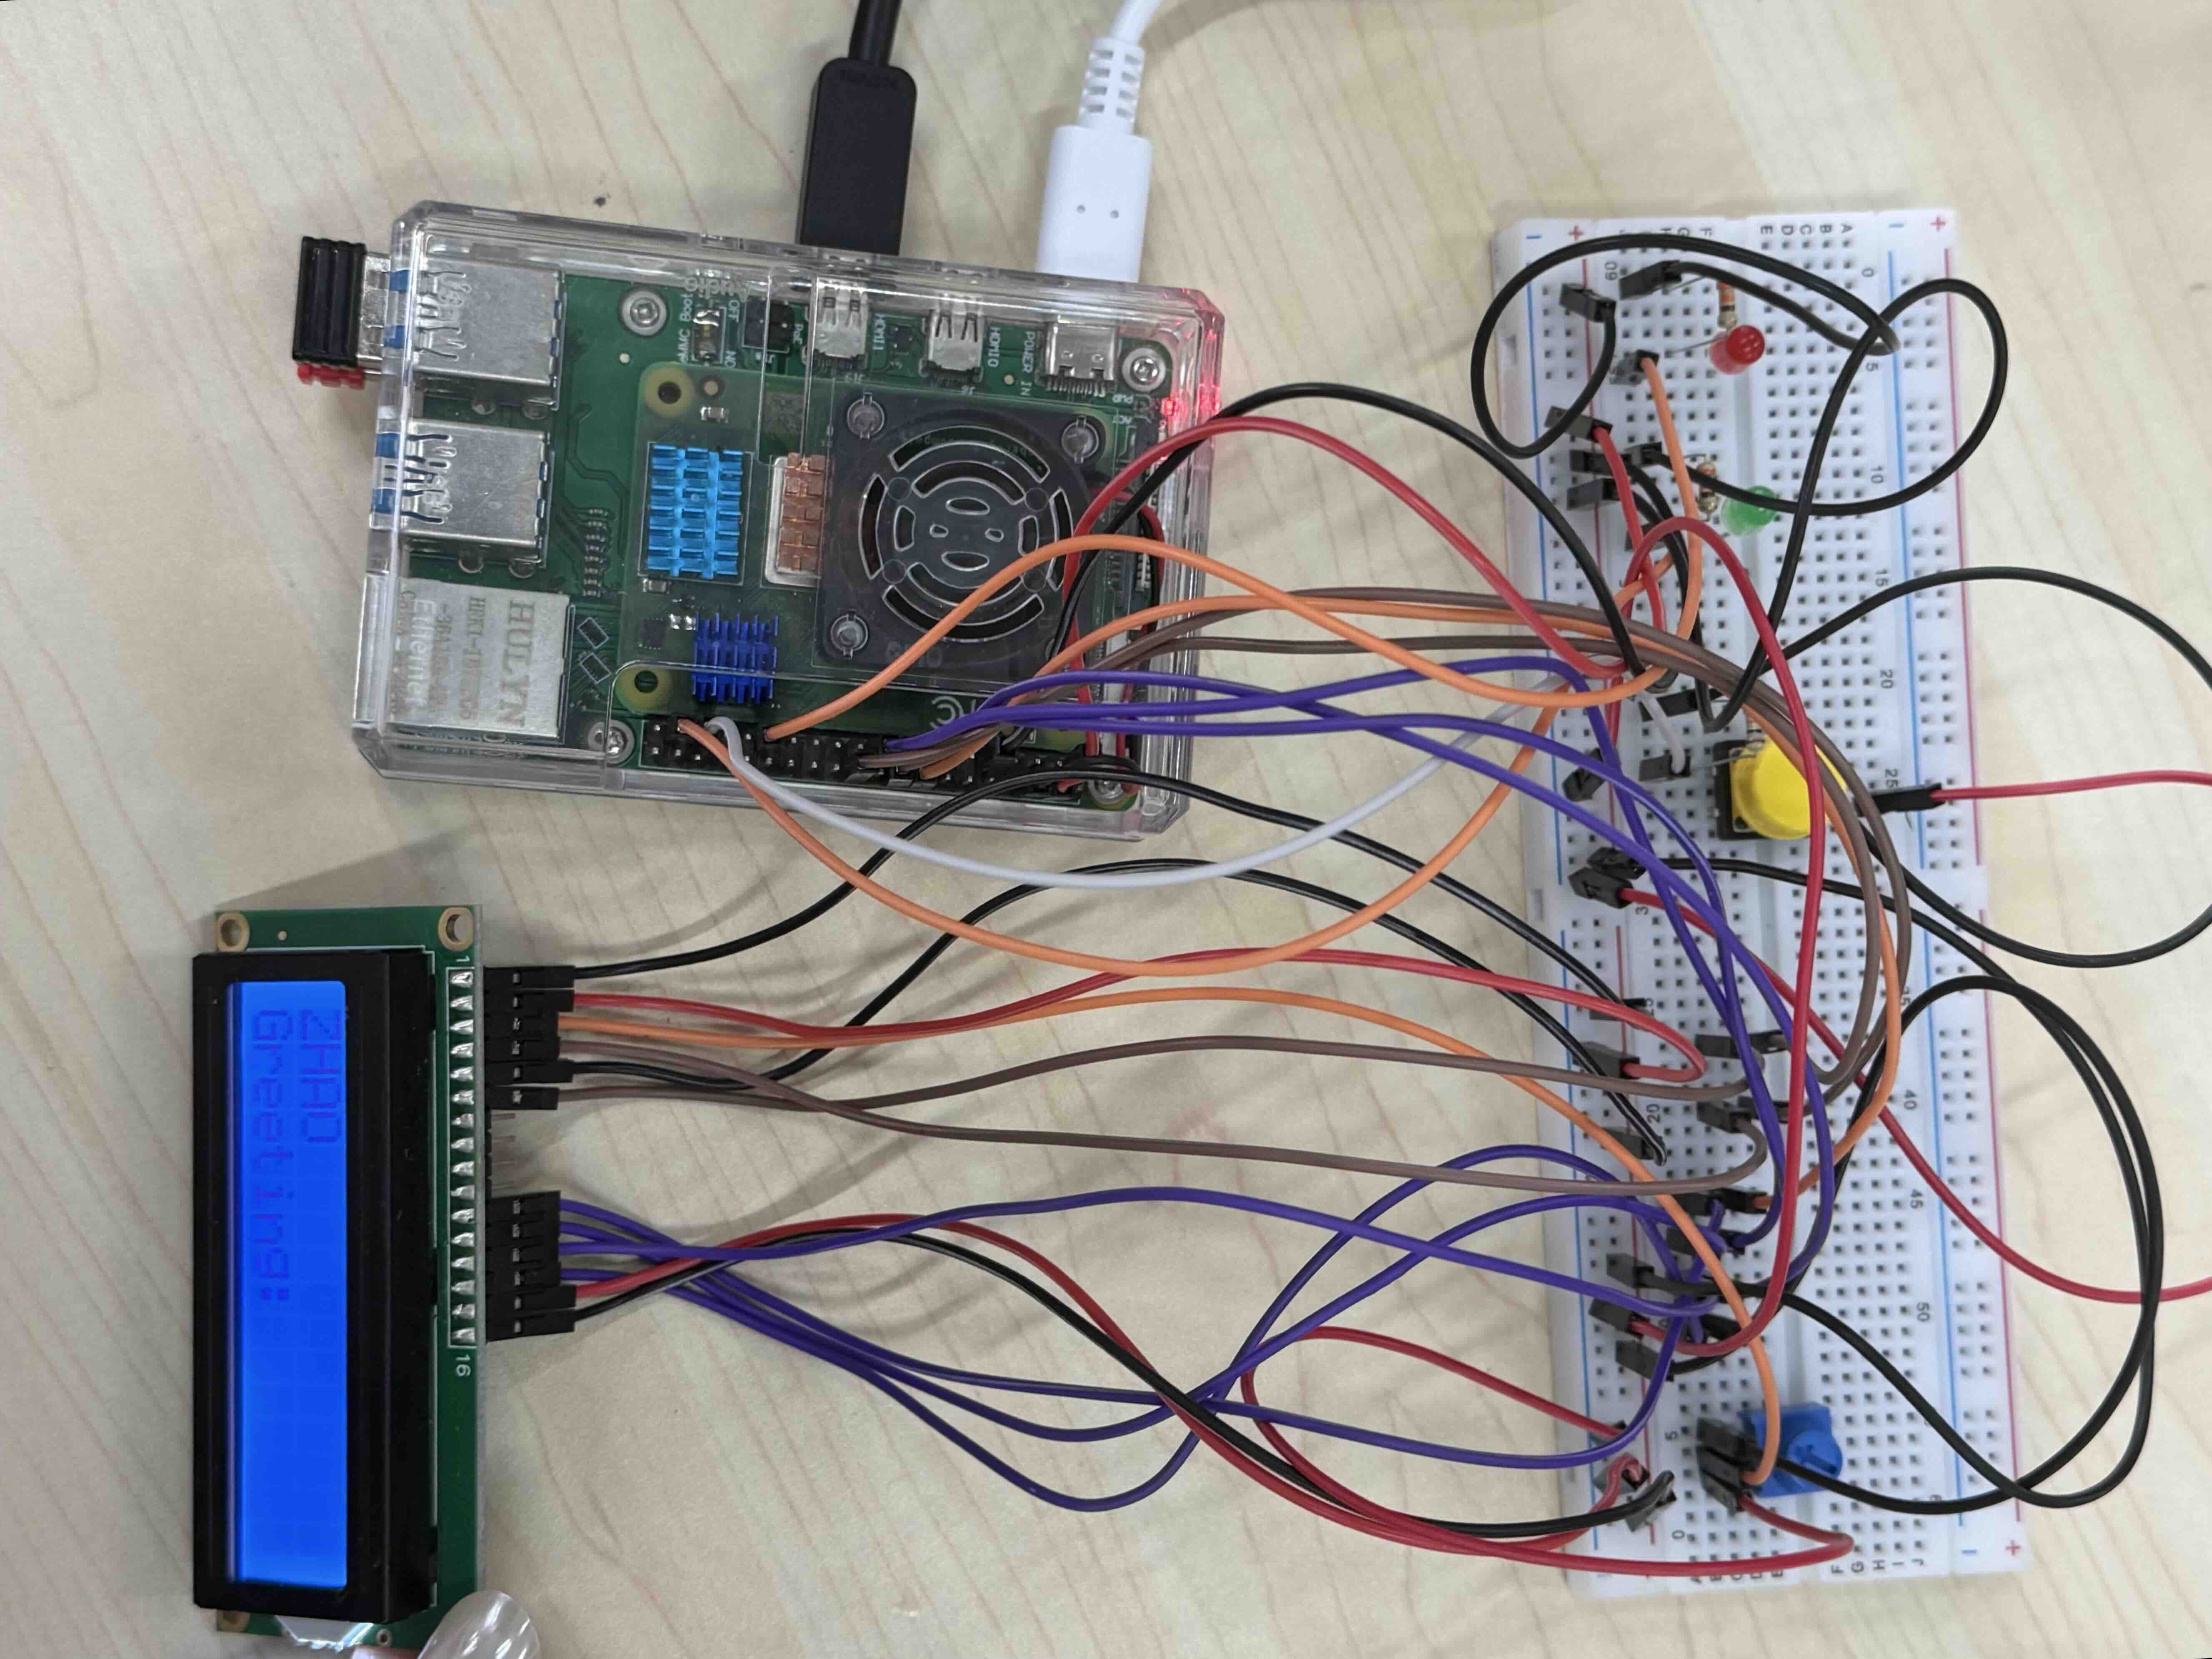
\includegraphics[width=0.8\columnwidth]{figures/hardware_wiring.jpg} 
    \caption{Schematic diagram of physical wiring.}
    \label{fig:wiring}
\end{figure}

The hardware platform of this project is Raspberry Pi, which runs a 32-bit system to ensure the compatibility of ARM assembly instructions. The external physical interaction system consists of several basic electronic components, including leds (red and green) for visual feedback, physical buttons for receiving user input, and an LCD display for displaying text information. In addition, a sliding rheostat is connected to dynamically adjust the contrast of the LCD display to ensure the visibility of the output information.

\vspace{-1em}

\begin{table}[H]
    \centering
    \caption{LED \& Button Configuration}
    \label{tab:led_button_config}
    \begin{tabularx}{\columnwidth}{@{}l l X@{}}
        \toprule
        \textbf{Modules} & \textbf{GPIO Pin} & \textbf{Function} \\
        \midrule
        Green LED   & GPIO 26   & Repeat user input and indicate successful search results. \\
        Red LED     & GPIO 5    & Status separation and input acknowledgment. \\
        Button      & GPIO 19   & Record the PIN sequence through timed presses. \\
        \bottomrule
    \end{tabularx}
\end{table}

\vspace{-1em}

All components are connected to the GPIO pins of the Raspberry Pi through the breadboard. The green led for data echo indication is connected to the GPIO 26 pin through a series 330$\omega$ resistor, and the red led for control signal and status separation is connected to the GPIO 5 pin. The physical button is plugged into a GPIO 19 pin and is configured in input mode in the system software for high-frequency polling to capture the user's actions.

\vspace{-1em}

\begin{table}[H]
    \centering
    \caption{LCD Display Configuration}
    \label{tab:lcd_config}
    \begin{tabularx}{0.75\columnwidth}{@{}l l X@{}}
        \toprule
        \textbf{LCD Pin} & \textbf{GPIO Pin} & \textbf{Function} \\
        \midrule
        1  (VSS)    & GND           & Ground                \\
        2  (VDD)    & 3V3           & Power Supply          \\
        3  (V0)     & Potentiometer & Contrast Adjustment   \\
        4  (RS)     & GPIO 25       & Register Select       \\
        5  (RW)     & GND           & Read / Write Control  \\
        6  (EN)     & GPIO 24       & Enable                \\
        11 (D4)     & GPIO 23       & Data Bit 4            \\
        12 (D5)     & GPIO 10       & Data Bit 5            \\
        13 (D6)     & GPIO 27       & Data Bit 6            \\
        14 (D7)     & GPIO 22       & Data Bit 7            \\
        15 (LED+)   & 3V3           & Backlight Anode       \\
        16 (LED-)   & GND           & Backlight Cathode     \\ 
        \bottomrule
    \end{tabularx}
\end{table}

\vspace{-1em}

For the most complex LCD display, we use 4-bits data transmission mode for wiring. The logic power supply (pin 2) and backlight power supply (pin 15) of LCD are connected to the 3v3 power supply of Raspberry Pi, and the ground pins (pin 1, 5, 16) are connected to the GND. The register select pin RS (pin 4) is connected to GPIO 25, the enable pin EN (pin 6) is connected to GPIO 24, and the read / write pin RW is directly grounded to lock the screen into write mode. LCD 4-bit data pins D4-D7 (pin 11-14) connect GPIO 23, 10, 27, and 22 of Raspberry Pi in turn, thus forming a complete and reliable underlying data transmission bus.

    \section{Division of Work}
\label{sec:work_division}

This coursework was developed collaboratively by Shijia Luo (H00460252) and Yuwei Zhao (H00460398). The specific contributions are as follows:

\begin{itemize}
    \item \textbf{Shijia Luo} is responsible for the hardware construction and the implementation of the basic I/O functions (Task 1-3).
    \item \textbf{Yuwei Zhao} is responsible for the implementation of the core cracking algorithms in C and ARM Assembly (Task 4-5).
    \item Both members participated in system testing and code review.
\end{itemize}

    \section{Code Structure \& Main Functions}
\label{sec:software_design}

The software architecture of this project follows the modular design principle of high cohesion and low coupling. The program uses C language as the main body, and the implementation separates hardware control from the cracking algorithm through modular functions. The whole code is composed of key modules like entry control, exception flow management, data initialization, verification simulation and core recursive search. The following are the main functions responsible for the core logic in the system and their functional details:

- \noindent \textbf{\texttt{main}} It is the core master function that drives the entire application. \texttt{getopt} was used to loop through complex command line parameters and parse out configuration information such as task mode, sequence length, delay parameter and whether to start exhaustive search. This function is responsible for preparing the hardware initialization by mapping the physical GPIO registers of the Raspberry Pi to the user space memory via \texttt{mmap}. The execution phase is mainly divided into three stages --- greeting display, button sequence input, and password cracking search. When the program terminates normally or catches an exception, the memory release and hardware state reconstruction are uniformly executed through a unique \texttt{cleanup} tag.

- \noindent \textbf{\texttt{initITimer} \& \texttt{timer\_handler}} These two functions work together to implement non-blocking hardware rotation using the interval timers of the Linux kernel. \texttt{initITimer} wraps the \texttt{setitimer} and \texttt{sigaction} system calls to start a timer that decrements real events. When a timer emits the \texttt{SIGALRM} signal, the kernel interrupts the current process and invokes the \texttt{timer\_handler} function to set the global timeout bit \texttt{timeout\_flag} to true. This design separates the time judgment logic from the high-frequency GPIO state reading, ensuring the time sensitivity and accuracy when reading the button input.

- \noindent \textbf{\texttt{initSeq} \& \texttt{readSeq}} These two functions are responsible for the generation and loading of PIN sequences in memory. \texttt{initSeq} exploits the random number generation of the system to generate secret sequences for the device to act as the target password and allocate them to the dynamic memory. \texttt{readSeq} takes the command line integer arguments, parses them bit by bit, and converts them into a standard array format. Simultaneously, it contains a check logic for out-of-bounds input, which ensures that the data structure is in a safe state before the algorithm is executed.

- \noindent \textbf{\texttt{submit\_pin}} In the real password cracking scenario, the password verification of the system is often associated with high computation or network delay. This function introduces a customizable blocking delay by calling \texttt{usleep} to simulate the verification cost. The underlying assembler is called to calculate the Hamming distance between the current guess sequence and the secret sequence, and then set it as the return value. This function is the only interface between the high-level search algorithm and the low-level decision logic.

- \noindent \textbf{\texttt{choose\_positions} \& \texttt{generate\_values}} These two functions constitute the core algorithmic components in Task 5 to cope with arbitrarily long sequence cracking. In order to solve the state space explosion problem caused by brute-force search, the program adopts the Hamming distance based pre-pruning and backtracking strategy. \texttt{choose\_positions} is the outer recursion that picks out all possible positions in the sequence based on the known Hamming distance. \texttt{generate\_values} is responsible for the inner recursion that enumerates all legal numeric changes at the selected index position. The two-level recursive method ensures that the program only generates valid candidate sequences that completely conform to the characteristics of Hamming distance, which fundamentally reduces the dimension of the search space and optimizes the performance.

The following snippet extracts the core validation logic of the inner recursive function and shows how it intercept the generation and submission of invalid states based on the Hamming distance:

\begin{minted}{c}
if (depth == code) {
    stats->attempts++;
    stats->submits++;

    int result = submit_pin(guess_seq, seqlen, submitDelay);

    if (result == 0) {
        stats->found = 1;

        if (stats->found_at == 0) {
            stats->found_at = stats->attempts;
            memcpy(stats->found_seq, guess_seq, seqlen * sizeof(int));

            LOG("PIN found: ");
            showSeq(guess_seq, seqlen);   
        }
    }
    return;
}
\end{minted}

In this code, the \texttt{submit\_pin} is called only if the recursion depth is equal to the target Hamming distance \texttt{code}, which avoids the traversal of useless search branches, significantly reduces the time complexity and achieves the using known information to optimize the cracking process.

    \section{Performance \& Resource Analysis}
\label{sec:performance_analysis}

In the PIN cracking scenario, the most significant performance bottleneck is the system latency incurred each time authentication is submitted in the form of blocked I/O inside the \texttt{submit\_pin} function. In order to maximize the efficiency, we optimize three aspects of the system --- algorithm architecture, os scheduling and underlying hardware interaction.

In terms of algorithm architecture, the program completely abandoned the resource-consuming naive brute-force search paradigm when dealing with the cracking task of arbitrary length sequences. The time complexity of brute-force search is as high as $O(D^N)$ (where \texttt{N} is the length of the sequence and \texttt{D} is the optional number base), which will lead to state space explosion in the case of long sequence and large base, extremely waste of CPU cycles and memory bandwidth. For this purpose, we use a constructive combinatorial search algorithm based on backtracking. It implements   a pruning by using the baseline Hamming distance returned by the initial reference sequence as an absolute constraint. The algorithm only deduces dynamically in memory and generates valid candidate sequences that strictly satisfy the Hamming distance characteristics of the target. The time complexity is dramatically compressed to $O(C(N,K) \times (D-1)^K)$ (where \texttt{K} is the known Hamming distance).

As for OS scheduling, exceptional control flow is introduced to optimize the resource consumption during I/O polling. The CPU-intensive timestamps are not used during the processing of button input to achieve accurate timeout detection with numeric separations. Instead, the system calls the interval timer \texttt{setitimer} of the Linux kernel and binds the \texttt{SIGALRM} asynchronous signal handler function, which enables the Raspberry Pi to effectively release resources to process other system-level tasks during the idle period of waiting for the user's key release or timeout, which greatly reduces the power consumption and unnecessary processor usage caused by single thread polling.

In terms of underlying hardware interaction and resource management, the program directly controls the physical hardware to minimize overhead. As will be detailed in the subsequent sections, implementing the high-frequency Hamming distance calculation in ARM assembly eliminates redundant instructions from high-level compilers. For GPIO control, mapping physical addresses via \texttt{mmap} and using inline assembly help to bypass library abstractions, ensuring microsecond I/O latency. Regarding memory, we avoid large static arrays; all sequence buffers are dynamically allocated based on the runtime \texttt{seqlen}. Task 5's recursive search bounds its maximum call stack depth to the target Hamming distance, which is typically much smaller than the total sequence length. This control over recursion, combined with on-demand memory allocation, effectively prevents stack overflows and maintains a minimal memory consumption when cracking extremely long sequences.

    \section{Hardware Access: C vs. Assembler}
\label{sec:hardware_access}

In this project, direct access to the underlying hardware of the Raspberry Pi (led, button, LCD display) is achieved through the memory-mapped I/O (MMIO) mechanism. In the initialization phase of the main program, the C language is used to call the \texttt{mmap} function to map the physical GPIO base address of the Raspberry Pi into the virtual memory space. In order to balance the flexibility of address calculation and the accuracy of underlying physical register operation, the program uses a mixed programming mode combining C and inline ARM assembly. There are three core functions that directly access the hardware, which are responsible for pin mode configuration, digital level output, and digital level input, respectively.

- \noindent \textbf{\texttt{pin\_mode}} It is used to configure a specific GPIO pin to input / output mode. The C language part is responsible for the arithmetic operation to calculate the \texttt{word\_offset} and the specific shift \texttt{fsel\_shift} of the GPIO Function Select register \texttt{GPFSEL} of the desired pin for the hardware design controls the mode of each pin by three consecutive bits. Then the inline assembler takes over and loads the GPIO base address into the \texttt{R2} register. It reads the current register value using the \texttt{LDR}, cleans the old mode bits by displacement using the \texttt{BIC}, writes the new mode mask passed in from C via the \texttt{ORR}, and writes the modified value back to the register using the \texttt{STR}, ensuring that only the specific pin is updated without affecting the settings of other pins sharing the same register.

- \noindent \textbf{\texttt{digital\_write}} It is used to control led on / off and send high / low levels to LCD data pins. C language is responsible for the conditional branch and addressing calculation, which determines whether to operate the pin set register \texttt{GPSET0} or zero register \texttt{GPCLR0} based on the passed level value HIGH / LOW and calculates the corresponding memory offset and the specific bitwise left shift. The inline assembler focuses on efficient writes at the hardware level and also follows the hard rules of storing the base address in the \texttt{R2} register. It utilizes the \texttt{LSL} to generate a mask containing only the target bit of 1 and writes data directly to the selected physical register via the \texttt{STR}. Since \texttt{GPSET} and \texttt{GPCLR} registers are designed so that writing a ``1'' triggers the action while writing a ``0'' has no effect and not interfere with each other on the hardware physical level, the assembly part directly eliminates the step of reading the original value, which improves the writing efficiency.

- \noindent \textbf{\texttt{read\_button}} It is used to high-frequency polling to read the current level status of the physical button. While the C logic of the function computes the address offset of the pin level register \texttt{GPLEV0} and the specific displacement of the desired pin in the 32-bit register, the inline assembler code uses the \texttt{LDR} to read the current system snapshot of the entire 32-bit pin level register after loading the physical base address into the \texttt{R2} register. The \texttt{LSR} was used to move the target bit logic right to the least significant bit \texttt{LSB}, \texttt{AND} was used to perform bitwise and operation with the constant 1, so as to separate the 0 / 1 state of the target pin, and return the variable assigned to the C language layer to the caller.

In order to show the collaborative working mode of C language and inline ARM assembly mode clearly, the following shows the specific implementation of \texttt{digital\_write} function, which reflects the communication between upper logical calculation and underlying physical address access.

\begin{minted}{c}
void digital_write (volatile uint32_t *gpio, int pin, int value) {
    int reg_offset = (value == HIGH) ? GPIO_GPSET0 : GPIO_GPCLR0;
    int word_offset = reg_offset + (pin / 32);
    int bit_shift = pin % 32;

    __asm__ volatile (
        "MOV r2, %[base] \n\t"              // load the raw GPIO base addr to R2
        "MOV r1, #1 \n\t"
        "LSL r1, r1, %[shift] \n\t"         // create bit mask
        "STR r1, [r2, %[off], LSL #2] \n\t" // write to GPSET/GPCLR
        :
        : [base] "r" (gpio), [off] "r" (word_offset), [shift] "r" (bit_shift)
        : "r1", "r2", "memory"
    );
}
\end{minted}

As shown in the preceding code, the C language is responsible for the hardware abstraction layer, which dynamically decides to manipulate the set / reset registers based on the incoming logic level state and precomputes the word offset and displacement. The subsequent inline assembler block receives these calculations as placeholders and enforces the underlying design constraint of storing the GPIO base address in the \texttt{r2} register in the first instruction \texttt{MOV r2, \%[base]}. The assembly part finally writes memory-mapped registers efficiently with a single \texttt{STR} via indirect addressing mode with logical left shift \texttt{[r2, \%[off], LSL \#2]}. This design not only ensures high execution efficiency, but also confirms the control over the characteristics of the target hardware architecture.

    \section{Hamming Function Interface}
\label{sec:hamming}

In this project, the calculation of Hamming distance is the core operation with the highest frequency and the most significant impact on the overall performance of the search algorithm. To ensure the efficiency and to apply low-level system programming, the function is encapsulated in an independent ARM assembly source file named \texttt{hamming.s}. Serving as the computational engine, this subroutine is called cross-language from the C main program to perform fast comparisons and count the differing bits between two equal length integer arrays.

In terms of interface definition and parameter passing, the prototype of C language exposed by the assembler function is an integer return function accepting two integer pointers and an integer length parameter. In the low-level implementation, the program strictly follows ARM Procedure Call Standard (AAPCS). In particular, when the assembler subroutine is invoked by the main program, registers \texttt{R0} and \texttt{R1} are implicitly allocated to hold the head address pointers of the first and second integer arrays to be aligned, respectively, and register \texttt{R2} is used to pass the current sequence length to be aligned. When the core comparison logic is executed, the Hamming distance calculation result, which represents the total number of unequal elements in the two arrays, is stored in the \texttt{R0} register and safely returned to the main call function with the jump of the program counter.

For the internal logic of subroutines, the assembly implementation adopts an efficient self-decreasing loop iteration structure. The subroutine saves the state of \texttt{R4}, \texttt{R5} and link register \texttt{LR} through the stack push instruction. In the main loop body, the program uses the \texttt{load} with the automatic post-increment mechanism to automatically move the pointer address back while reading the current element of the memory array, which reduces the addressing overhead. The core comparison decision completely depends on the conditional execution characteristics of ARM instruction set. The program first updates the subtraction status flag of the elements in the two registers, and then directly uses the unequal status code to perform conditional addition.

In order to show the above mechanism, the core code implementation of the assembly subroutine is extracted as follows:

\begin{minted}{c}
.global hamming
	
hamming:
    PUSH {R4, R5, LR}
    MOV R3, #0

loop_start:
    CMP R2, #0
    BEQ loop_end

    LDR R4, [R0], #4
    LDR R5, [R1], #4

    CMP R4, R5
    ADDNE R3, R3, #1

    SUB R2, R2, #1
    B loop_start

loop_end:
    MOV R0, R3
    POP {R4, R5, PC}
\end{minted}

As shown above, the \texttt{R3} register is allocated to be used as a local accumulation counter. The loop terminates when the residual length register \texttt{R2} decrements to 0. Finally, the program transferred the accumulated Hamming distance results in \texttt{R3} to the specified return value register \texttt{R0}, and recovered the original context through the stack operation and returned to the C language running environment exactly. 

    \section{Application Output \& Testing}
\label{sec:application_output}

In this section, a series of specific command-line test cases are used to verify the pin-cracking application. All the tests are directly run on the Raspberry Pi, aiming to verify the correctness and efficiency of the system design through real runtime data.

In order to verify the basic state flow, parameter parsing ability, and simulation verification mechanism of the program, we first execute:

\vspace{0.5em}

\begin{minted}{bash}
sudo ./cw2 -v -d -S 500000 -s 312 -r 112
\end{minted}

The detailed output snapshot validates the command-line parser by accurately applying the 500,000-microsecond delay and bypassing hardware input via a reference sequence. Furthermore, the terminal output confirms the underlying cracking logic's correctness by demonstrating the complete lifecycle, from the initial Hamming distance calculation to the successful target sequence capture.
%附录改
See Appendix Fig \ref{app:fig8_1} for the corresponding test result.

The second test is about performing a black-box verification on ARM assembly subroutine responsible for calculating Hamming distance. 

\begin{minted}{bash}
sudo ./cw2 -e -u -s 112 -r 121
\end{minted}

As illustrated in the Appendix Fig \ref{app:fig8_2}, the program calculates a Hamming distance of 2 between sequence 112 and reference 121, verifying the accuracy of underlying register alignment logic for cross-language data interaction.
%附录改

To evaluate the computational efficiency of the system when dealing with sequences of arbitrary length, exhaustive performance tests were run:

\begin{minted}{bash}
sudo ./cw2 -e -n 6 -m 12 -s 123123 -r 111123
\end{minted}

The environment extends the sequence length to 6 bits, the maximum of each input is increased to 12, and the exhaustive mode is enabled. 
See Appendix Fig \ref{app:fig8_3} for the corresponding test result.

The output clarifies the node to find the target sequence, and it shows the complete running trace of the program without early termination. The data shows that with the pruning of the constructive combinatorial search algorithm, the system accurately locks the number of expensive submit verifications that is 1,816 times, and the overall running time is only about 0.16 seconds. This confirms the performance analysis strategy about reducing the search space and memory dynamic management mentioned above.

    \section{Conclusions \& Reflections}
\label{sec:conclusion}

This project successfully achieved all the requirements of the coursework, and constructed a complete and stable Raspberry Pi software and hardware interaction system. In terms of basic functions, the program directly controls the physical keys, LED indicators and display through the underlying code, and properly handles the timeout problem when the user input. In the core cracking logic, the system not only uses efficient basic assembly instructions to complete the comparison calculation of password differences, but also implements an intelligent derivation algorithm for arbitrary length passwords. All expected tasks have passed rigorous system testing.

The highlight of our project lies in its system optimization and integration of hardware and software. In terms of hardware, fast response is achieved by directly manipulating memory addresses. As for algorithm, the system uses logical investigation and advance filtering instead of blind brute force testing, which fundamentally avoids the computing power collapse that may be caused when long passwords are cracked. At the same time, the program insists on applying memory to the system on demand, and strictly controls the resource occupation during the running process, which perfectly adapts to the objective reality of the limited hardware capabilities of embedded devices.

Through this system programming practice, we have a deeper understanding of the software and hardware co-development. It significantly helped to improve our ability to write low-level instructions and learn how to manage memory more safely and precisely in C. More importantly, this assignment helped us establish a global system thinking, that is, we learned how to transform the complex software logic into efficient and stable bottom execution actions step by step with limited physical resources, which laid a solid foundation for the future engineering development.

    \appendix  % 开启附录模式
    

% 附录图 1
\begin{figure}[h]
    \centering
    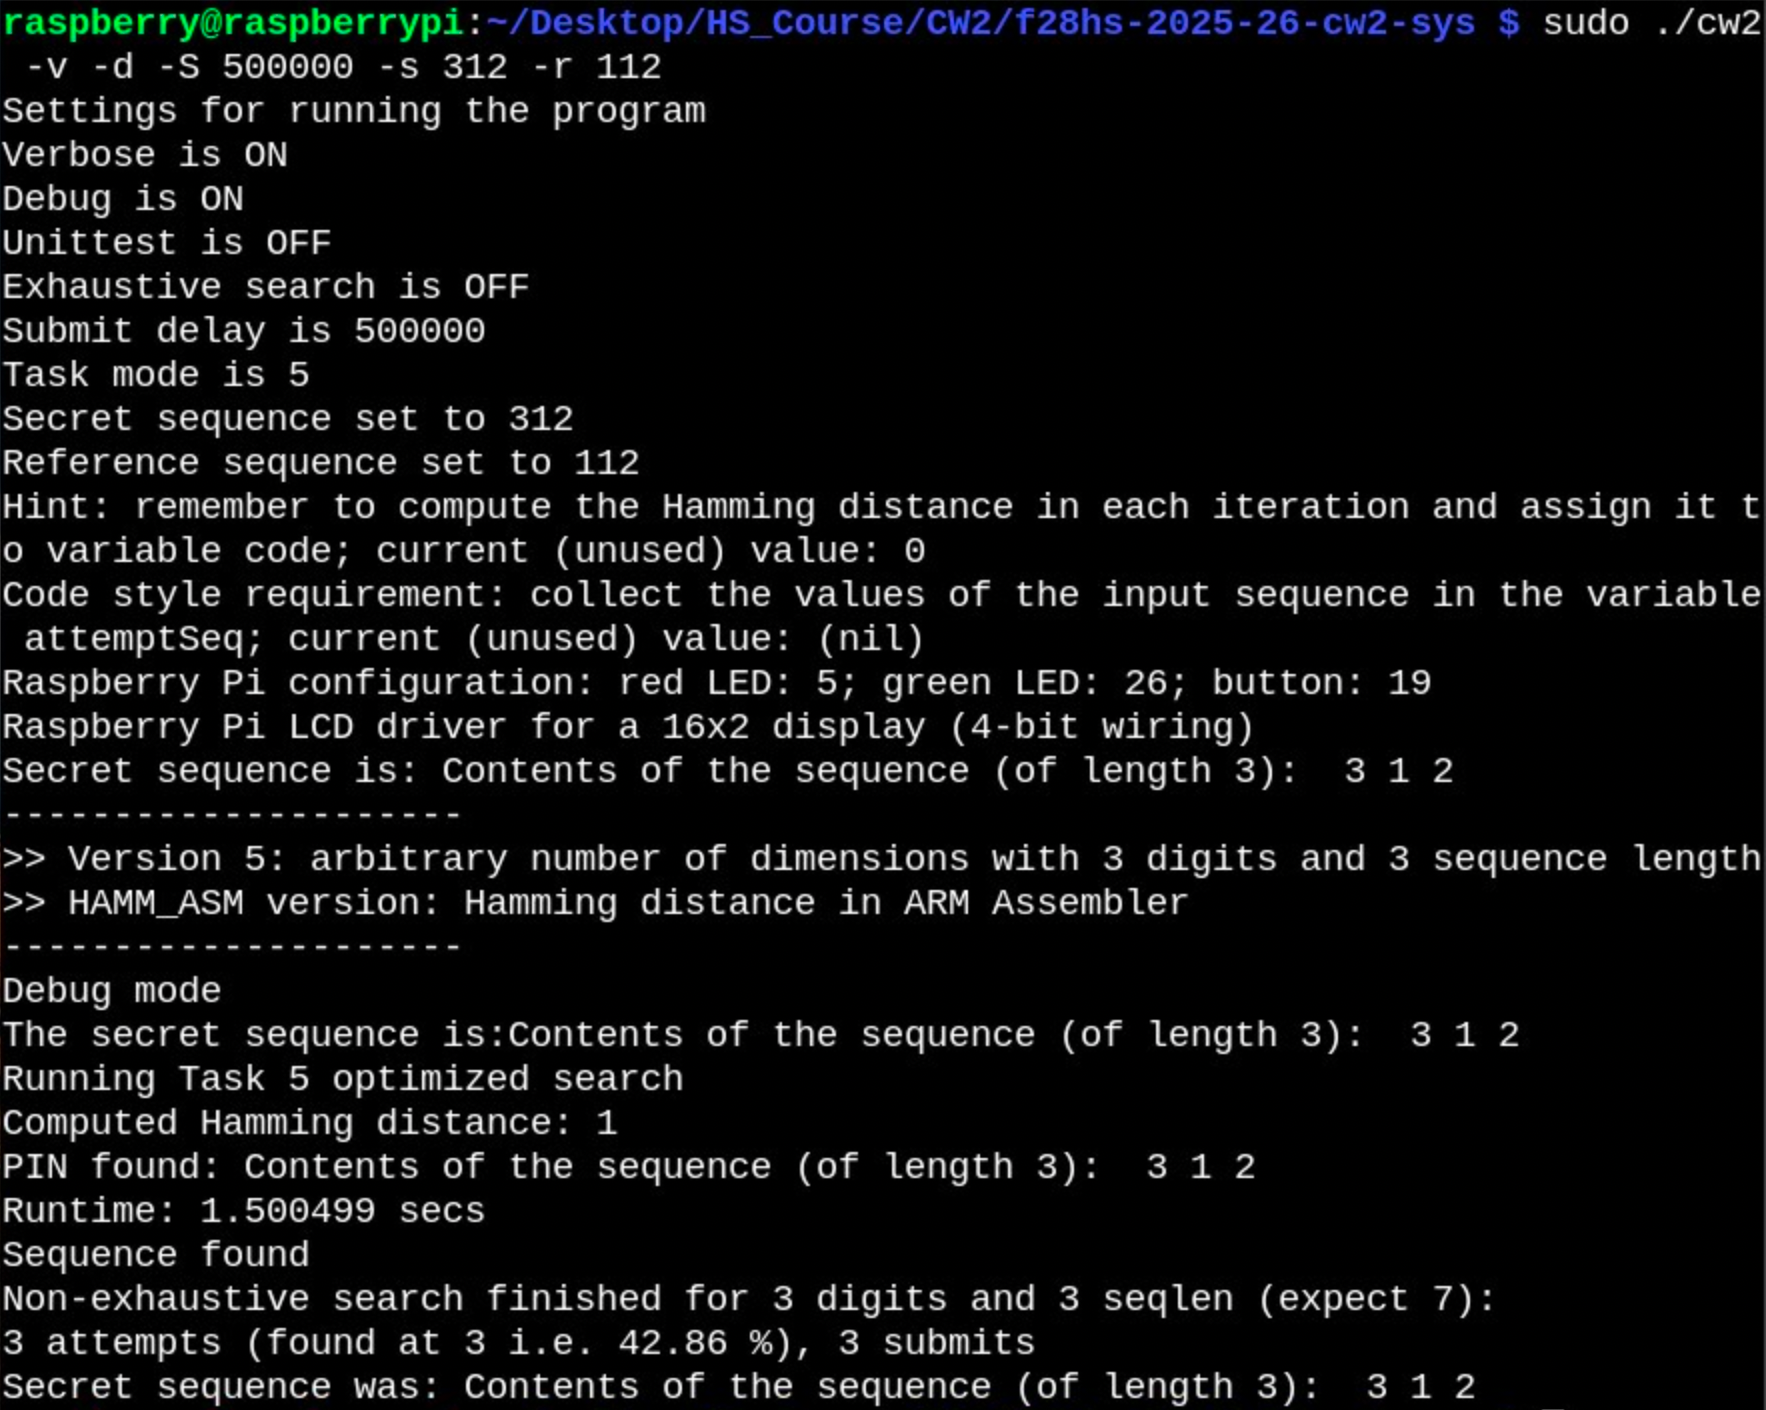
\includegraphics[width=0.8\linewidth]{figures/figure_81.png}
    \caption{Test results of base control flow and detailed configuration output.}
    \label{app:fig8_1}
\end{figure}

% 附录图 2
\begin{figure}[h]
    \centering
    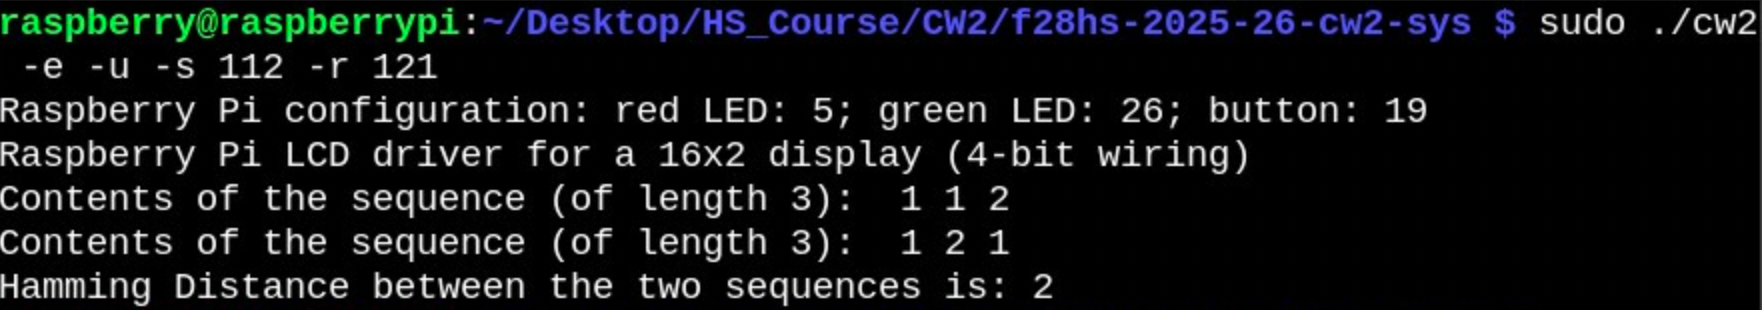
\includegraphics[width=0.8\linewidth]{figures/figure_82.png}
    \caption{Test results of Hamming distance calculation.}
    \label{app:fig8_2}
\end{figure}

% 附录图 3
\begin{figure}[h]
    \centering
    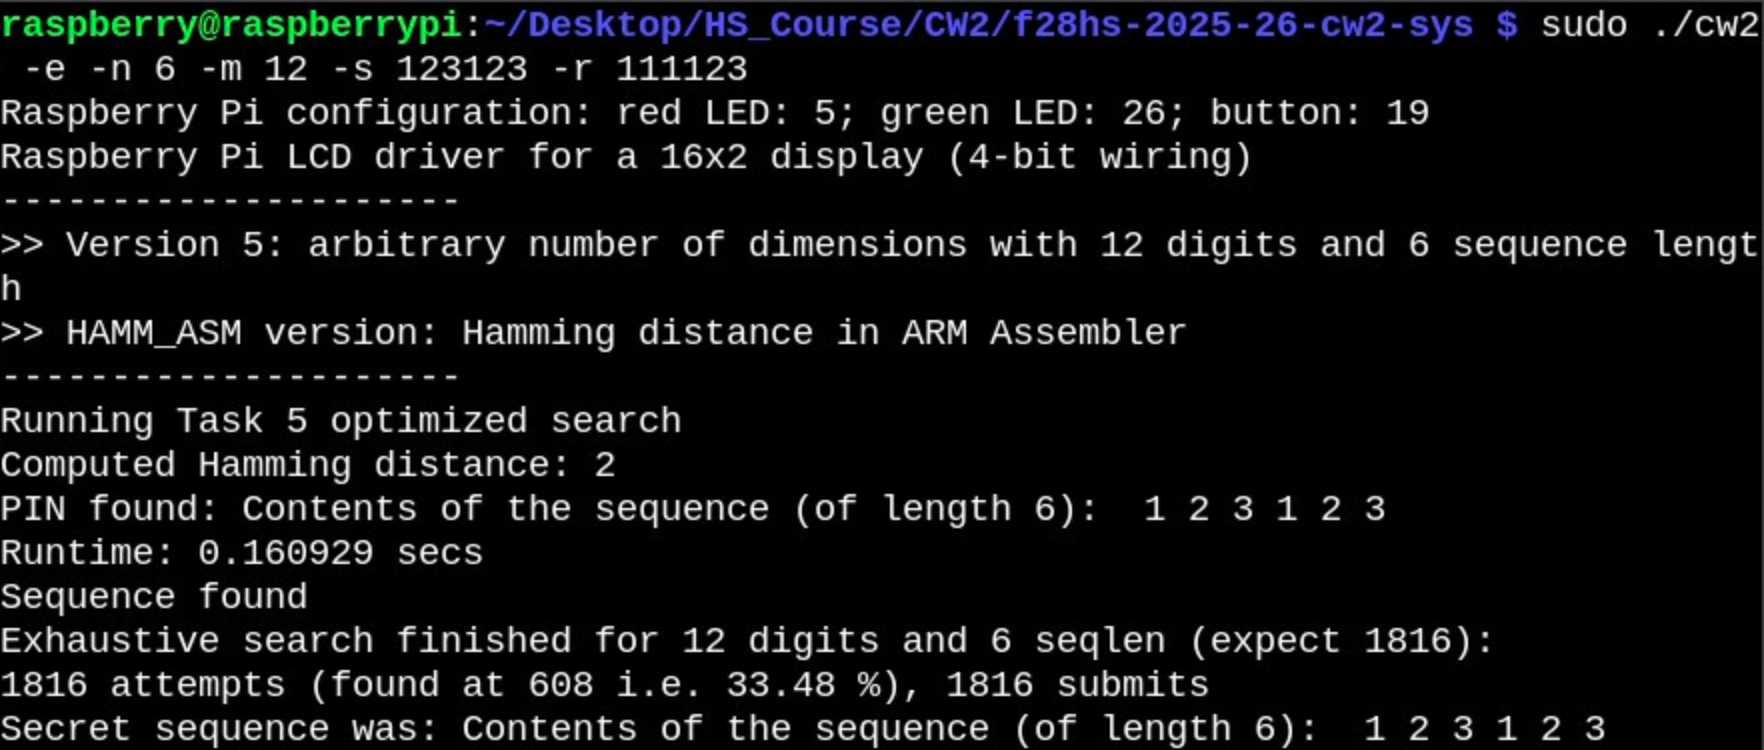
\includegraphics[width=0.8\linewidth]{figures/figure_83.png}
    \caption{Test results of constructive combinatorial search and exhaustive performance for arbitrary length sequences.}
    \label{app:fig8_3}
\end{figure}  % 你的附录内容
\end{document}
